\begin{figure}[H]
  \centering
  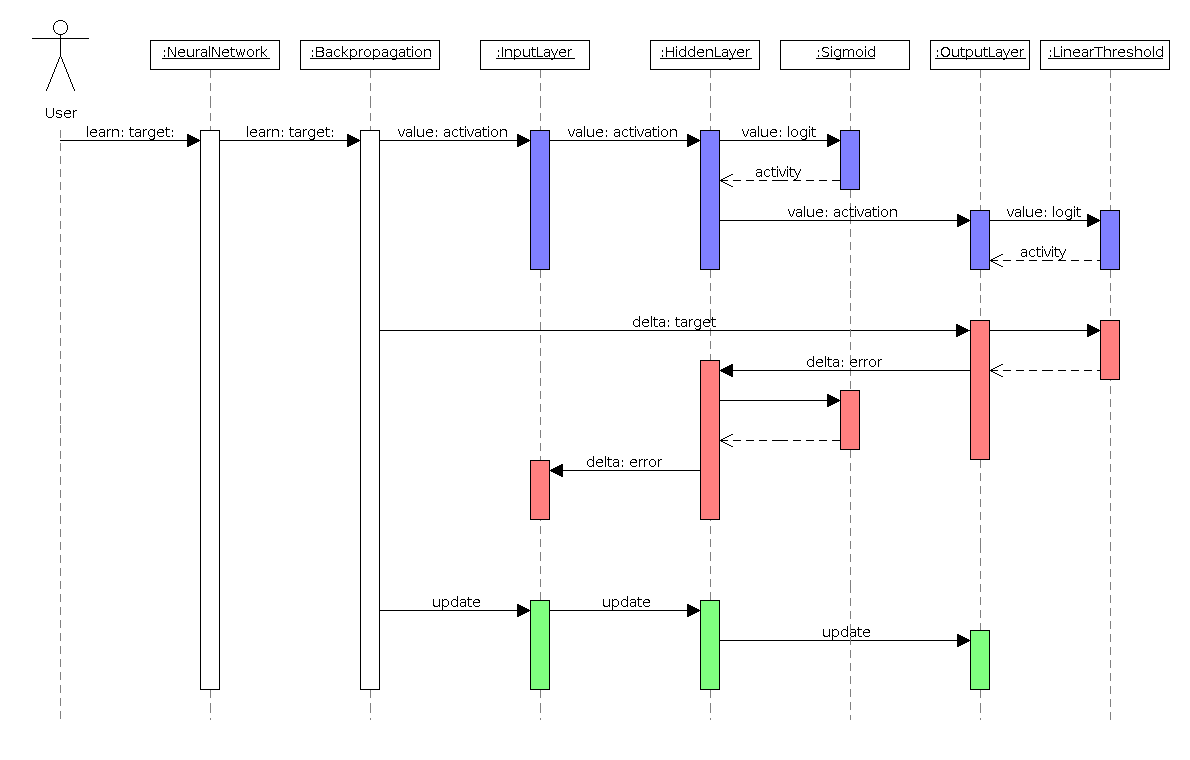
\includegraphics[width=\linewidth]{backprop_seq}
  \caption{Implementing activation functions as methods of specific subclasses on Neuron}
  \label{fig:backprop_seq}
\end{figure}

\subsection{LearningAlgorithm class: Strategy Pattern}
Backpropagation is the most widely used algorithm for training multi-layer neural networks. But not the only one. There are many other algorithms available, such as… . Though, at this point I will not be implementing anything except backpropagation, I don’t want to force it onto the user and make him redesign half of the framework in order to use some other algorithm.

But even backpropagation comes in different forms. It can be update the weights after each training example (online) or after looking at a whole dataset (batch). The most efficient though is the one that looks at smaller subsets of a training data before updating the weights (mini-batch). Generally speaking, these are types of learning, and they don’t affect the idea of backpropagation. But the learning algorithm as a sequence of actions changes a lot:

\begin{quote}
Online: forward - backward - update - forward - backward - update ...
Batch: forward - backward - forward - backward - ... - update
\end{quote}

Another way in which implementations of backpropagation can be different is how the learning rate is chosen. The easiest solution is to let the user pick a constant learning rate, and keep it unchanged for the whole period of learning. It is not a very good approach, because:

\begin{enumerate}
  \item It can be very hard to choose a good learning rate. If it is too small, the learning will be too slow - the network will need thousands of epochs to reach some relatively good performance. If the learning rate is too big, the algorithm will eventually start diverging - the cost will be growing, meaning that the performance is only getting worse.
  
\begin{figure}[H]
  \centering
  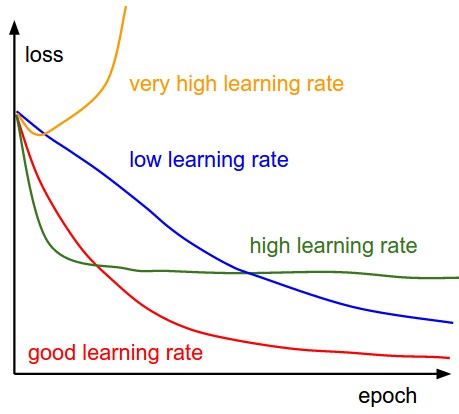
\includegraphics[width=\imgwidth]{learningrates}
  \caption{The demonstration of how the change of a learning rate affects the process of learning}
  \label{fig:learningrates}
\end{figure}
  
  \item (Batch learning) At the beginning, when we start from some random position in a weight space, we can be really far from the desired optimum. We want our learning rate to be big enough, so that we can get relatively close to that optimum in as little steps as possible. But as we get closer, we want to reduce our learning rate, in order to approach the optimum more slowly. Otherwise we may “jump too far” and start diverging.
  
\begin{figure}[H]
  \centering
  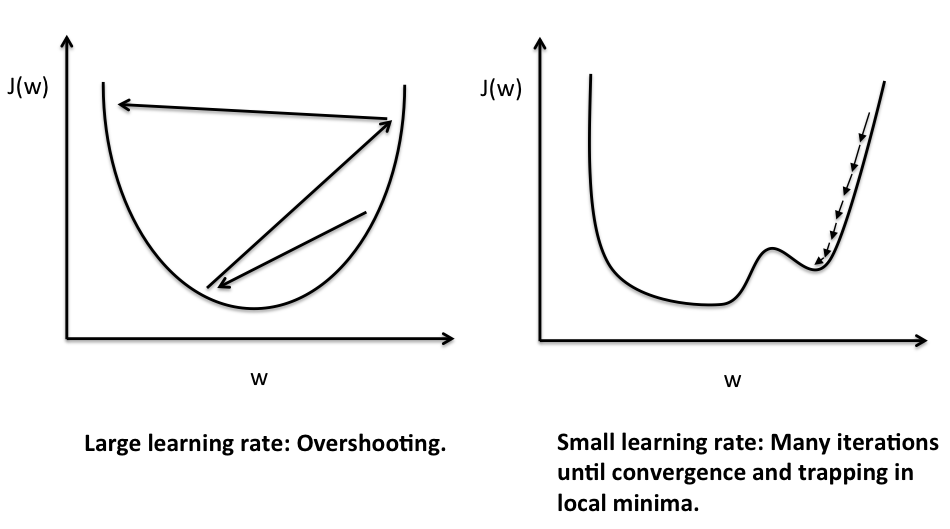
\includegraphics[width=0.75\linewidth]{learningrate_problems}
  \caption{Different types of problems when choosing a learning rate}
  \label{fig:learningrate_problems}
\end{figure}
  
  \item When it comes to multi-layer neural networks, the surface of a cost function in a multidimensional weight space that we are trying to optimize, becomes very complex and highly nonlinear. It may have many local optima in which we may get stuck with a small learning rate. We may need an algorithm that would increase the learning rate every time we get into the local optimum.
\end{enumerate}

\begin{figure}[H]
  \centering
  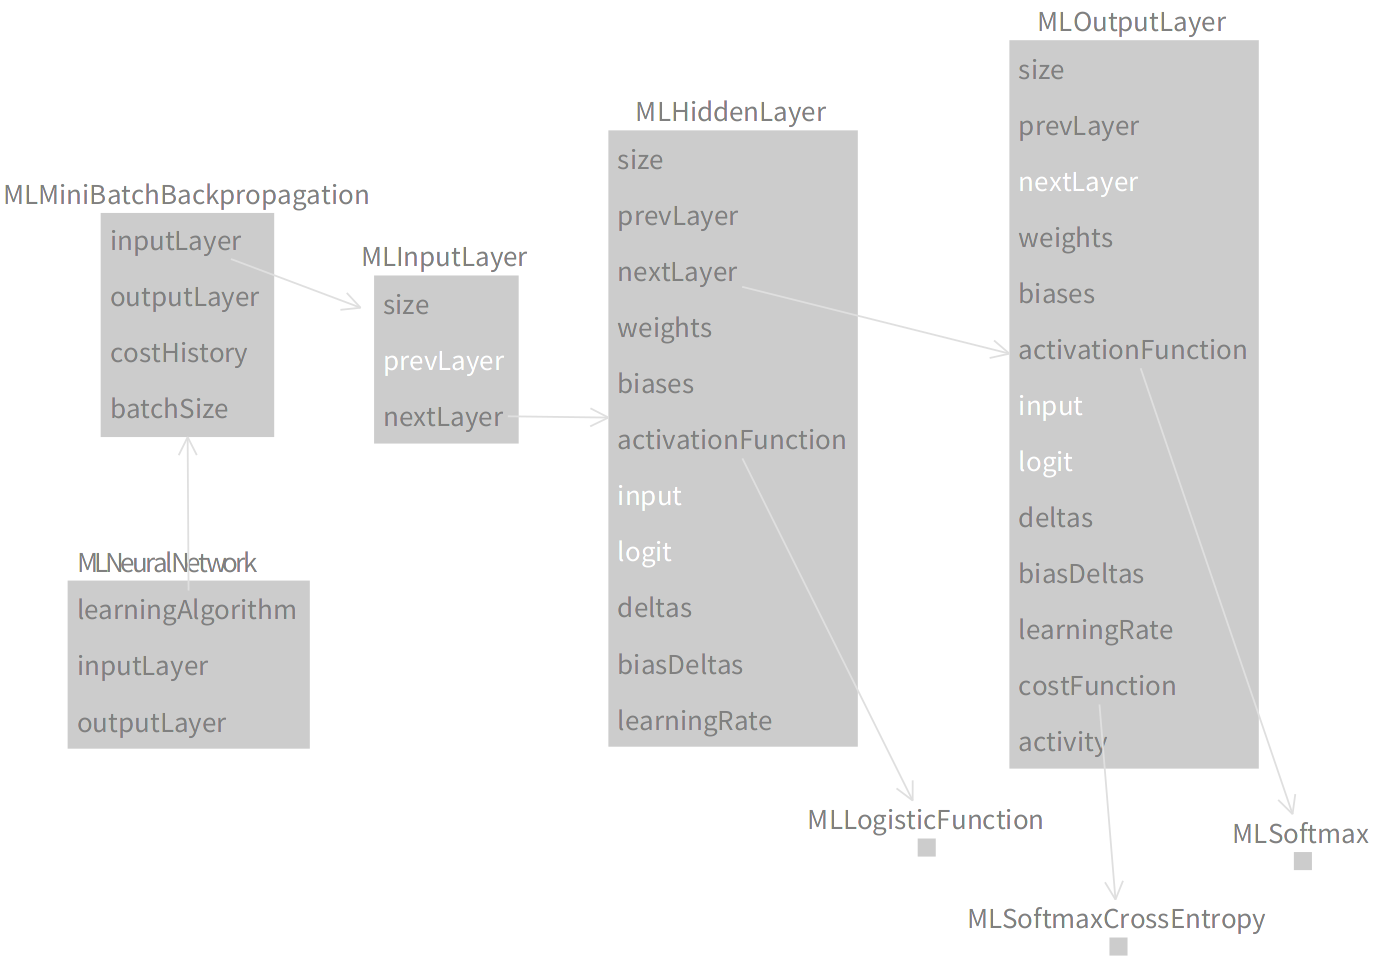
\includegraphics[width=\imgwidth]{objects}
  \caption{The graph of connections between the objects. Not all connections are visualized}
  \label{fig:objects}
\end{figure}

\subsection{Weight initialization}
Neural network is a machine learning algorithm that changes its weights to improve the performance on a given dataset. Each configuration of weights represents a point in the multidimentional space. The process of learning is based on minimizing the cost function, defined on that weight space. Therefore, setting the initial weights means choosing the starting point for the process of minimization. If the initial weights are close enough to the global minimum (best set of weights), the learning will be fast. If they are far - the network will take a lot of time to learn, or fail to converge at all.

Initializing all weights with zeroes is the easiest thing to do. However, a network with such weights may never learn anything. All weight updatades $\Delta w$ will be equal to zero.

It is recommended to initialize the weights with a small random values. Initializing a network with random weight can be a massive boost in performance. Pinto et al.\cite{Pinto-et-al-2008} evaluated thousands of architectures on a number of object recognition tasks and found that random weights performed only slightly worse than pretrained weights. And \cite{Saxe-et-al-2011} showed that while random weights are no substitute for pretraining and finetuning, their use for architecture search can improve the performance of state-of-the-art systems. 

According to \cite{Trushevskyi-2014}, a good way to initialize the weights of a layer $L$ is by choosing random values from range $\big[-\frac{1}{2k}, \frac{1}{2k}\big]$, where $k$ is the number of neurons in layer $L$.
